
\documentclass[12pt]{article}

        \usepackage{graphicx}
        \usepackage{booktabs}
        \usepackage{fullpage}
        \usepackage{hyperref}
        \usepackage{subfig}
\usepackage[T1]{fontenc}
\usepackage{cprotect}
\usepackage[depth=4]{bookmark}


\begin{document}

\tableofcontents
\section{Executive Summary}
This report analyzes the data collected in the data challenge files for signal being `Noisy' or `non-Noisy'. We find that a Logistic Regression classifier is able to obtain 0.89 AUC with 8 features. Tuning the classifier's decision threshold may be used to operate in different regimes, in this example we have chosen to operate at maximum balanced accuracy by using a decision threshold of 0.39.

\begin{enumerate}
\item{Data sources: CSV files given as part of challenge, with labeled time series data. }
\end{enumerate}


\section{Data exploration}
To begin, the data exploration component consists largely of visual inspection of the datasets time series results to generate ideas for feature generation. One finding here to flag is that we find that the labeling appears visually to be not very different between the positive and negative labels. That is, time series information is often qualitatively the same between the two channels when viewed as a normalized time series. In addition, the nature of the positive labels appears to be different from that demonstrated in the initial problem statement, see \ref{fig:spikes}. In Figure \ref{fig:exploration} we see a visual comparison of the two classes, after min-max normalization. The vertical offset is simply to better visualize independent charts. 

\clearpage

\begin{figure}
\centering
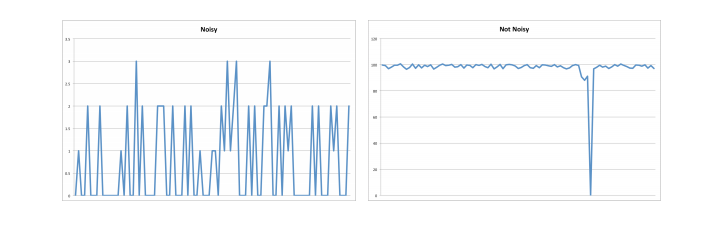
\includegraphics[width=1\textwidth]{spikes.png}
\caption{Description of noisy and non-noisy samples in the explainer document. }
\label{fig:spikes}
\end{figure}

\begin{figure}
\centering
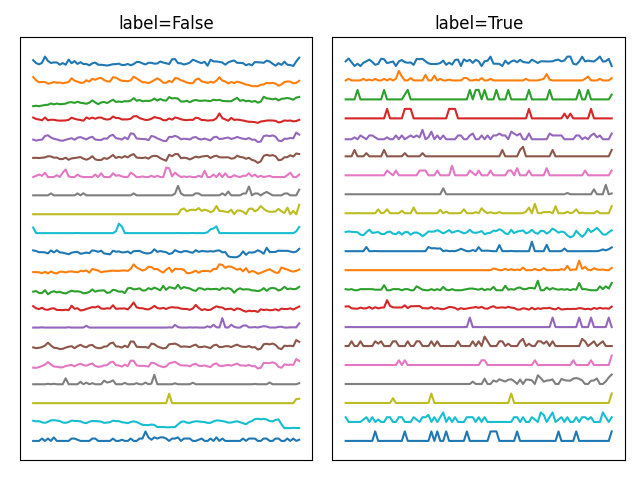
\includegraphics[width=1\textwidth]{exploration.png}
\caption{Raw time series plots from the two classes. The data is range normalized for better visual comparison. We see many qualitative similarities between the two labels.}
\label{fig:exploration}
\end{figure}
\clearpage
\section{Features}
For features, based on the time series in Figures \ref{fig:spikes} and \ref{fig:exploration}, we consider the following major categories:
\begin{enumerate}
\item{FFT based features - decomposes time series signal into discrete frequency components. This transformation is often sensitive to certain types of time series information such as spikes, different periodicity}
\item{Regression based features - fits a simple linear line to the data, either standard Linear Regression or regressions less sensitive to outliers such as the Theil-Sen regressor. This transformation is expected to be useful for signals with a bias, or fluctuations which are biased to positive or negative trend, or extreme fluctuations in baseline behavior (spikes, etc). }
\end{enumerate}
These basic remappings of the data are then collapsed further by a variety of methods appropriate for statistical distributions such as basic mean, median, range, quartile concentrations, and standard deviation, skew, and kurtosis. A large number of features are generated programmatically by the code in \verb|exploration.py|, with the generated features recorded appropriately in the column name of the resulting dataframe. 

\subsection{Feature selection}
By producing combinations of features, such as algebraic combinations of features, more features are generated than we have data for. Therefore, feature selection will be an important aspect of the project. All things being equal, we prefer to use fewer features in the final model. In the final findings, we present a combination of individual and product features, then use Sequential Backward Selection to map out the behavior of the model to the test data. This is done by executing the file \verb|ml_sbs.py|. We use the Logistic Regression Classifier in the SBS algorithm. The final performance point is shown in the right hand side of figure \ref{fig:sbs}. 
The resulting features list is the following, which gives an average ROC AUC score of 0.89.
\begin{enumerate}
\item{Signal concentration in the upper tail $>$ 0.25, RANSAC Regressor Residual}
\item{Signal concentration in the upper tail $>$ 0.01, Linear Regressor Residual}
\item{Ratio(Signal concentration in frequency weighted FFT $<$ 0.05, Signal concentration in frequency weighted FFT $<$ 0.2)}
\item{Ratio(Signal concentration in lower tail $<$ 0.05, Theil-Sen Regressor Residual, Signal concentration in lower tail $<$ 0.25 Theil-Sen Regressor Residual)}
\item{Ratio(Signal concentration in upper tail $>$ 0.1, Theil-Sen Regressor Residual, Signal concentration in lower tail $<$ 0.01, Linear Regressor Residual)}
\item{Ratio(Signal concentration in lower tail $<$ 0.01, Linear Regressor Residual, Signal concentration in upper tail $>$ 0.01, Theil-Sen Regressor Residual)}
\item{Ratio(Signal concentration in lower tail $<$ 0.2, Weighted FFT, Signal concentration in lower tail $<$ 0.05, Theil-Sen Regressor residual)}
\item{Ratio(Signal concentration in lower tail $<$ 0.2, Weighted FFT, Signal concentration in lower tail $<$ 0.01, Linear Regressor residual)}
\end{enumerate}

\paragraph{Comment} When the backward selection algorithm is taken all the way to one feature, the following single feature has a cross validation scores (ROC-AUC) of 0.76. 
\begin{enumerate}
\item{Ratio(Signal concentration in lower tail $<$ 0.2, Weighted FFT, Signal concentration in lower tail $<$ 0.01, Regression residual)}
\end{enumerate}


\begin{figure}
\centering
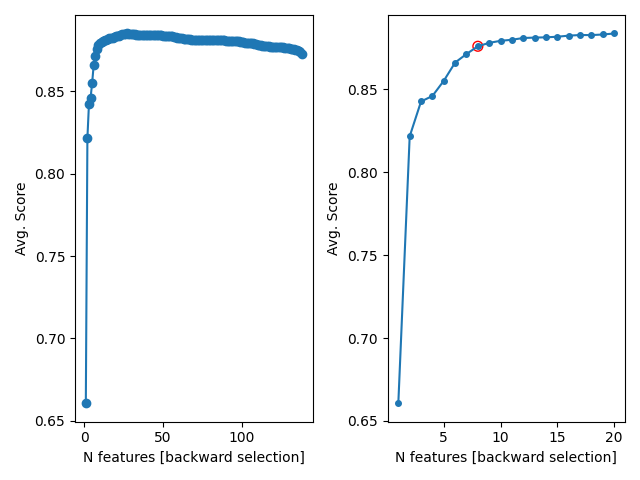
\includegraphics[width=1\textwidth]{ml_sbs_avg_score_products.png}
\caption{Sequential Backward Selection curves from the large list (137 features) down to 1 feature. We pick the point with 8 features as the point to operate the classifier. }
\label{fig:sbs}
\end{figure}
\section{Model performance}
In this section we look at final tuning and detailed performance of the Logistic Regression classifier used in the SBS feature selection algorithm. Using the raw feature crunching from \verb|exploration.py| $\rightarrow$ \verb|features.csv| and the feature list from the SBS algorithm \verb|ml_sbs.py| $\rightarrow$ \verb|final_columns.csv|, we execute the final training and evaluate performance on the test set. 

The learning curve is presented in Figure \ref{fig:learning}. We see a continued improvement in the classifier as the number of training samples increases. However, the presence of a gap between the training and validation curves suggests that some hyperparameter tuning via regularization may be beneficial. 

The out of the box performance in terms of confusion matrix is shown in Figure \ref{fig:base-cm} at decision threshold of 0.5. The model performance on the test set is show in Figure \ref{fig:performance}, with variation in the decision threshold from 0 to 1. Using this, we select the best model based on the balanced accuracy metric, though this could be adjusted in practice based on the application and preference for false positives vs false negatives. The resulting ROC curve is shown in Figure \ref{fig:roc}, again with decision point highlighted. 

Finally, we look at the confusion matrix of this classifier on the test set, compared to a random classifier (weighted by the labelled class distribution) in Figures \ref{fig:random} and \ref{fig:tuned}. We see a modest improvement over the random classifier, doubling the number of positive samples correctly detected. Further improvements may be obtained by looking at other classifiers, a wider range of features (we considered a subset of possible features here due to computational requirements), and tuning hyperparameters such as the regularization strength. 

\section{Conclusions}
In this report we have taken the data challenge time series data set through a basic machine learning pipeline. We have produced infrastructure for generating a large number of features based on the time series, which have shown to give modest improvement over a random classifier. Further efforts would be spent on (1) understanding the nature of the features used in the model in order to hypothesize more features (2) further efforts to identify improved classifiers and (3) hyperparameter tuning. Finally, the business context of the classifier performance needs to be established to be able to better suggest a model to deploy to production (e.g. in order to maximize business value). 


\begin{figure}
\centering
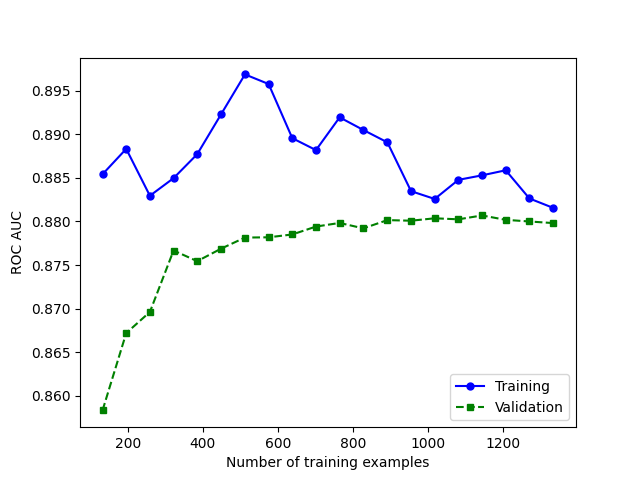
\includegraphics[width=1\textwidth]{learning.png}
\caption{Learning curve for Logisic Regression Classifier}
\label{fig:learning}
\end{figure}

\begin{figure}
\centering
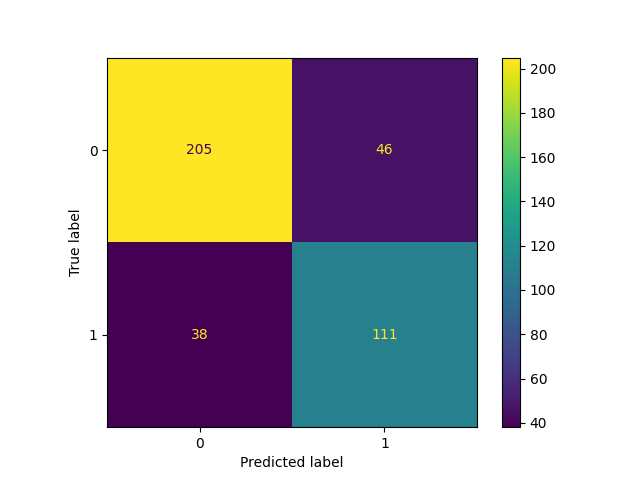
\includegraphics[width=1\textwidth]{cm0.png}
\caption{Confusion matrix for out of the box classifier}
\label{fig:base-cm}
\end{figure}
\begin{figure}[ht]
\centering
\subfloat[Performance curves for Logisic Regression Classifier and the operating point at decision threshold 0.39 is highlighted. ]{\label{fig:performance}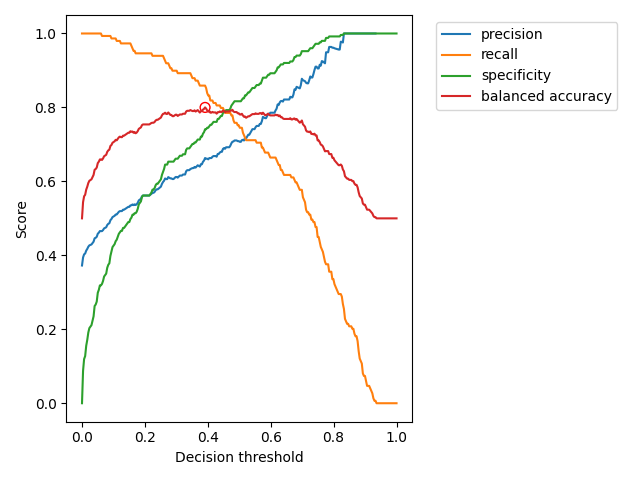
\includegraphics[height=6cm]{performance.png}}\hfill
\subfloat[ROC curve for Logistic Regression Classifier, and the operating point at decision threshold 0.39 is highlighted.]{\label{fig:roc}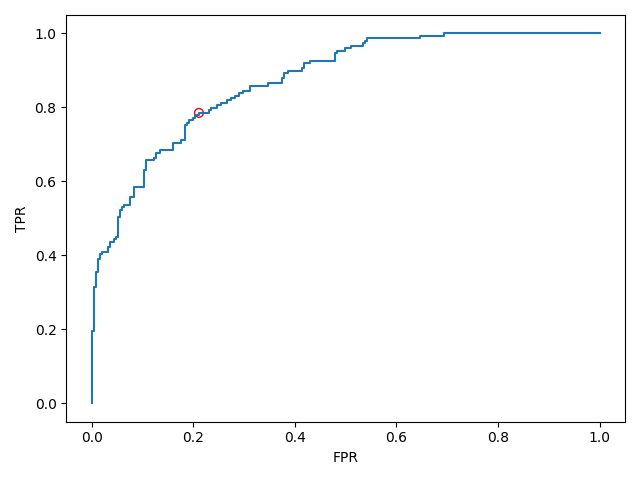
\includegraphics[height=6cm]{ROC.png}}\\

\caption{Performance comparison charts vs decision threshold. The operating point is taken at the point of maximum balanced accuracy}
\end{figure}
 
\begin{figure}[ht]
\centering
\subfloat[Random classifier (weighed by class proportion)]{\label{fig:random}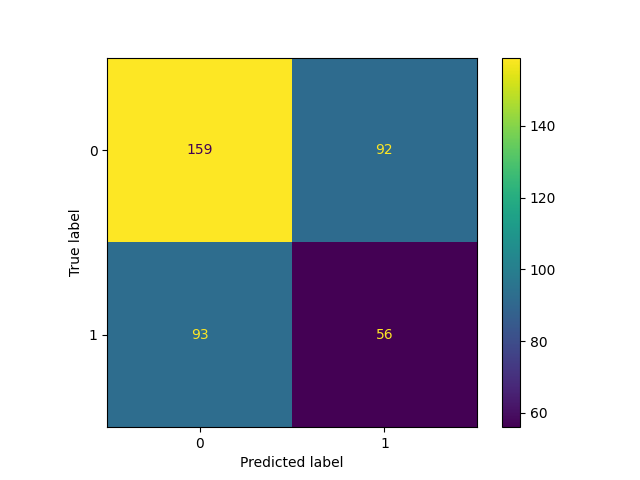
\includegraphics[height=6cm]{cm_random.png}}\hfill
\subfloat[Logistic regression classifier operating at decision threshold 0.39]{\label{fig:tuned}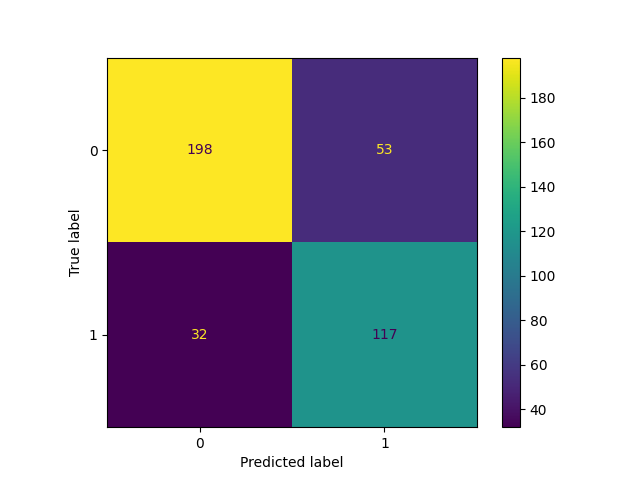
\includegraphics[height=6cm]{cm_tuned.png}}\\

\caption{ROC comparison}
\end{figure}
 
\end{document}
    